

\chapter{Semantic segmentation}
\label{chapter:unet}

\begin{introduction}
In this chapter we will present the second technique used to detect archaeological sites, semantic segmentation.
\end{introduction}

Identifying objects in images can be achieved by various methods, not limited to object detection alone. While object detection involves placing a bounding box to detect the object, there are alternative approaches such as instance segmentation and semantic segmentation. These methods aim to classify the image at the pixel level by assigning a class to each individual pixel within the image.

The goal of instance segmentation is to classify and distinguish individual objects in an image. In this method, each pixel is given a classification of which class it belongs to. In addition, each object is assigned to an individual class, which makes it possible to distinguish between objects of the same class. In this way, instance segmentation provides detailed information about the location and class of each object.

Semantic segmentation, on the other hand, focuses only on classifying the class of the pixel, without distinguishing between different objects of the same class. In this method, the image is divided into semantically meaningful regions, and each pixel within a region is assigned to the same class.

The next image illustrates the difference between semantic segmentation and instance segmentation.

\begin{figure}[H]
\centering
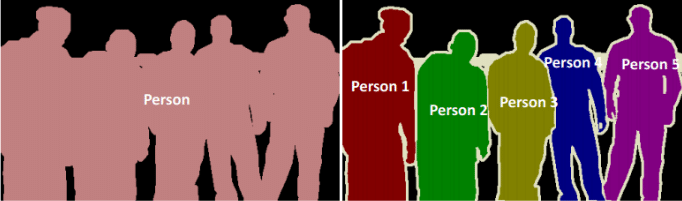
\includegraphics[width=10cm]{images/semanticVSinstance.png}
\caption{Semantic segmentation VS Instance segmentation \cite{semanticvsinstance}}
\end{figure}


Both instance segmentation and semantic segmentation require first predicting the instances of objects and their binary masks. It is done object detection and then semantic segmentation. The existing methods are generally divided into two categories\cite{instayolo}, two-stage and one-stage instance segmentation.

The two-stage methods generally involve object detection, obtaining the bounding box of objects followed by obtaining the mask within each bounding box. This is how for example MaskRCNN works, this algorithm uses Faster R-CNN to get the bounding boxes and then adds a new branch to get the segmentation.

The one-stage methods, on the other hand, perform detection and segmentation directly without getting the bouding boxes.

Following these two methods, an example of each was used, for the two-stage method YOLOv7-seg was used, and for the one-stage one Unet was used.




\section{Unet}
Unet is a neural network widely used in semantic image segmentation tasks, having been proposed in 2015, it is where today one of the most popular neural networks for semantic segmentation.

The main motivation behind Unet was the challenge of medical image segmentation\cite{unetpaper}.
In constrast of the previous model, Unet gives one classification for each pixel.

Unet's architecture consists of two parts: the encoder and the decoder. The encoder is composed of convulse and polling layers, which reduce the resolution of the input image, and filter image features. These features are then passed to the decoder, which performs upsumpling and concatenation operations. It is because of these U-shaped downsampling and upsampling operations that the architecture is called Unet.

\begin{figure}[H]
\centering
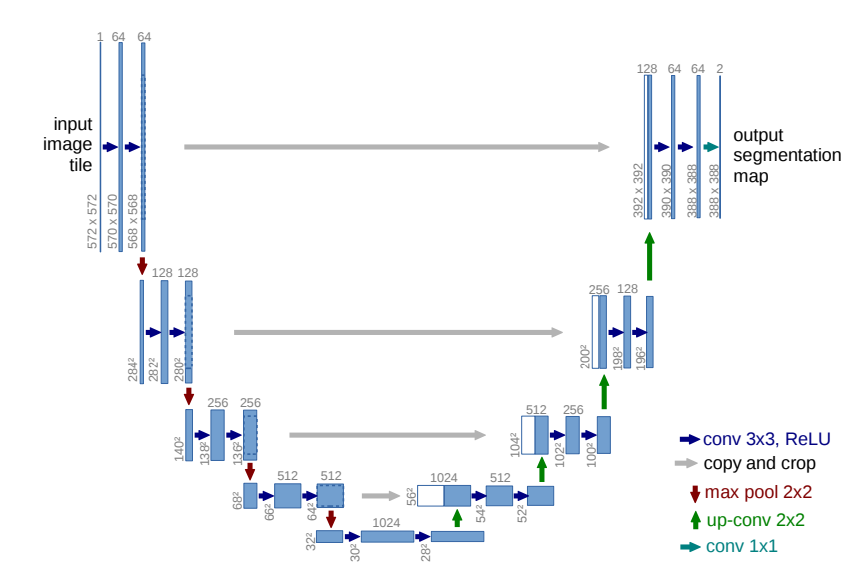
\includegraphics[width=15cm]{images/unetarquitetura.png}
\caption{Unet's architecture\cite{unetpaper}}
\end{figure}

\subsection{Model training}
In order to train the Unet model it was used the implementation present in the repository\cite{unetRep}. The repository already provides a pre-trained model trained with the carvana dataset.

The training dataset used was the same for YOLOv7. However, unlike YOLO, the annotations in Unet are not in text format, but in image format. To adapt the dataset, a Python script was created to read the annotations with the segmentations created during the dataset creation process and transform each text file into an all-black image with the object masks blank.

The next image shows a photo of the dataset copy paste of hillforts and its generated label.

\begin{figure}[H]
    \centering
    \subfloat{{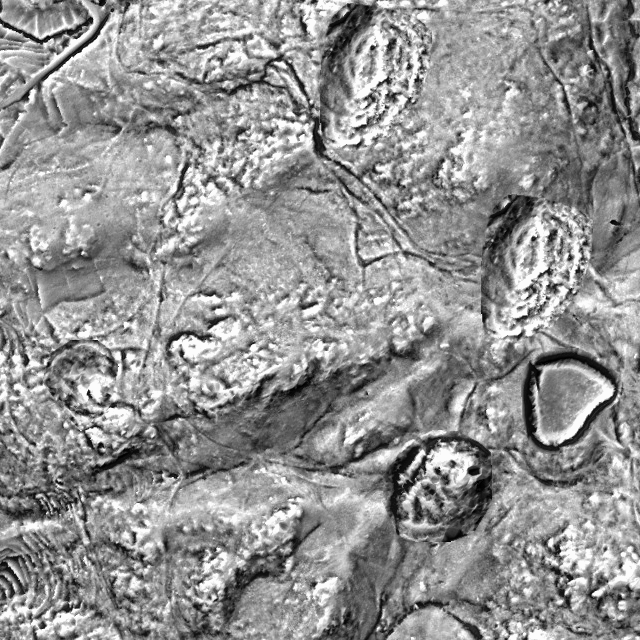
\includegraphics[width=7cm]{images/datasetExemples/seg/image.png} }}%
    \qquad
    \subfloat{{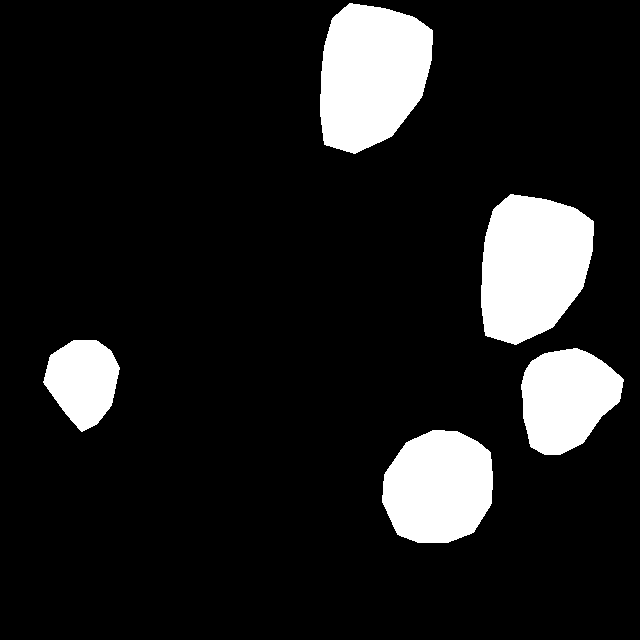
\includegraphics[width=7cm]{images/datasetExemples/seg/mask.png} }}%
    \caption{Example of label for Unet training}%
\end{figure}

The training script has also been adapted to save the best generated model of all seasons. Also, an early stop was added so that if there is no improvement in 40 seasons, the training will stop.

The metric validation dice was used to evaluate the training. The Dice index (also known as the Dice coefficient) is a widely used metric for evaluating the overlap or similarity between two image segmentation masks. It is often used in segmentation problems, such as the segmentation of objects in medical images. It is calculated based on the comparison between the segmentation mask predicted by the model and the reference mask (ground truth). The calculation of the Dice index involves counting the corresponding pixels in the two masks and comparing the intersection and the sum of the areas of the masks.

The dice index is given by the following formula:

\begin{equation}
    Dice = \frac{2 \times \text{Area of Overlap}}{\text{Total Area of Mask 1} + \text{Total Area of Mask 2}}
\end{equation}

The value of the Dice index ranges from 0 to 1, where 0 indicates no overlap between the masks and 1 indicates perfect overlap. The closer the Dice value is to 1, the better the overlap between the masks and therefore the better the segmentation quality.

The next images show the evolution of the dice index during the training process.

\begin{figure}[H]
\centering
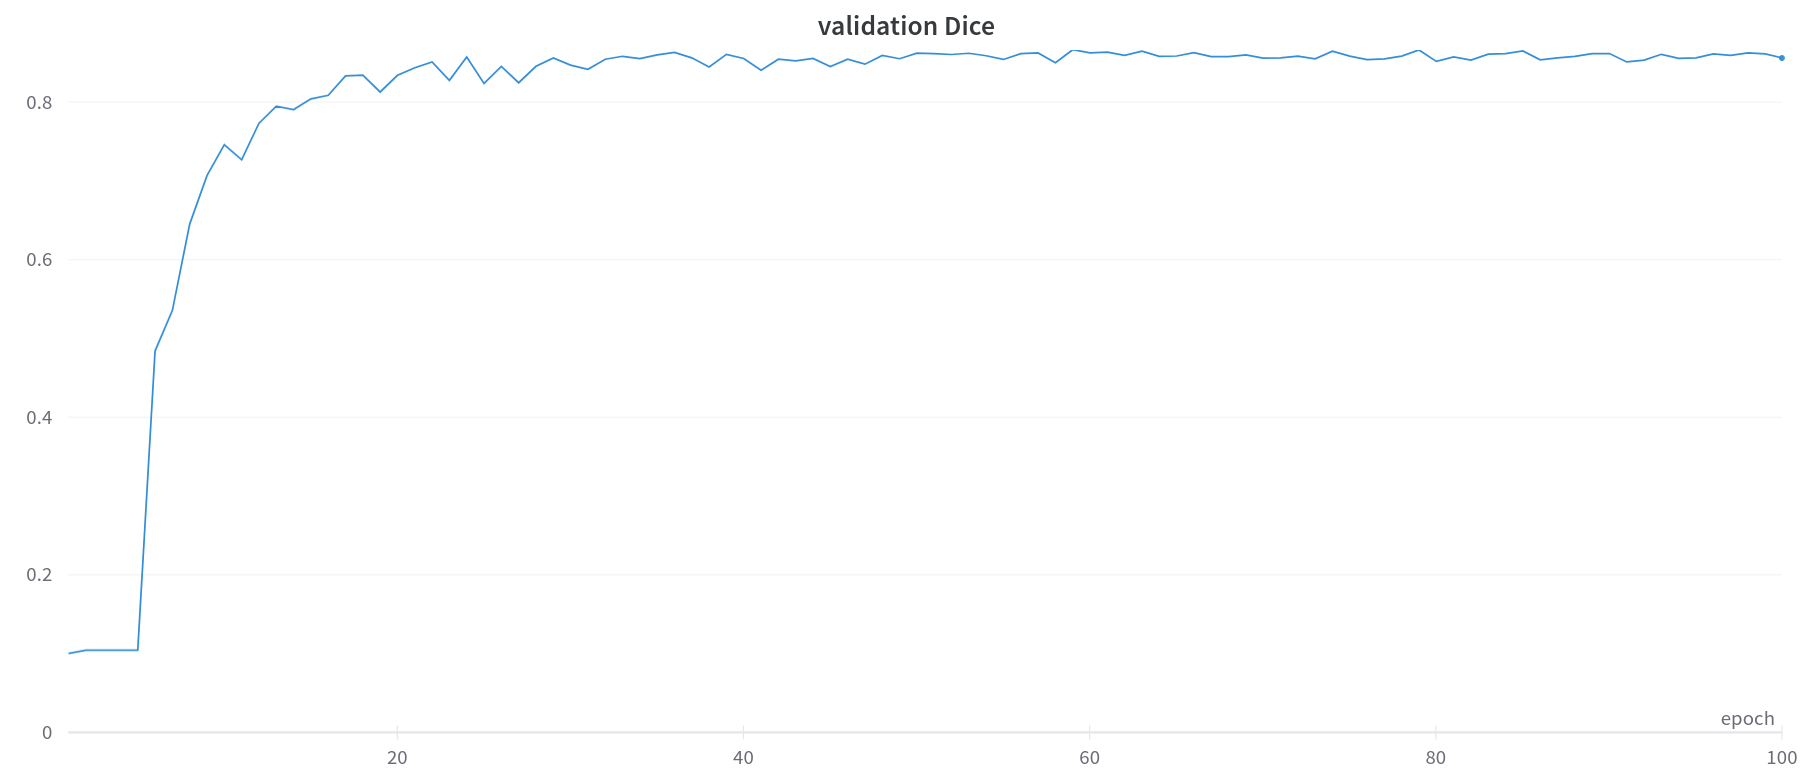
\includegraphics[width=12cm]{images/unet/mamoas_copy.png}
\caption{Evolution of dice index for tumulis copy paste dataset}
\end{figure}

\begin{figure}[H]
\centering
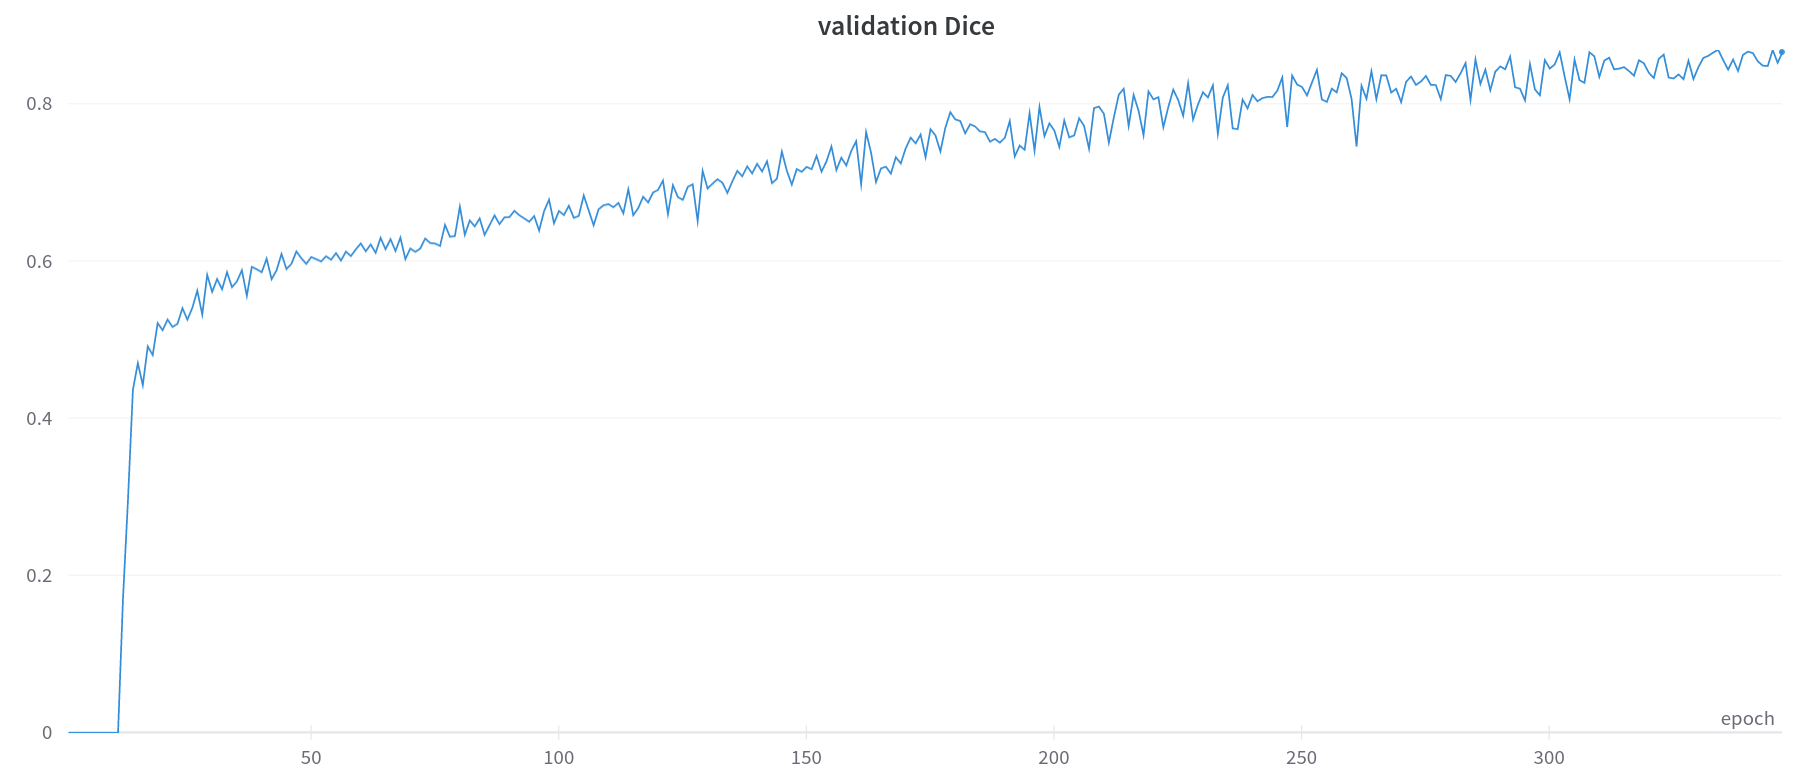
\includegraphics[width=12cm]{images/unet/mamoas_simple.png}
\caption{Evolution of dice index for tumulis simple dataset}
\end{figure}

\begin{figure}[H]
\centering
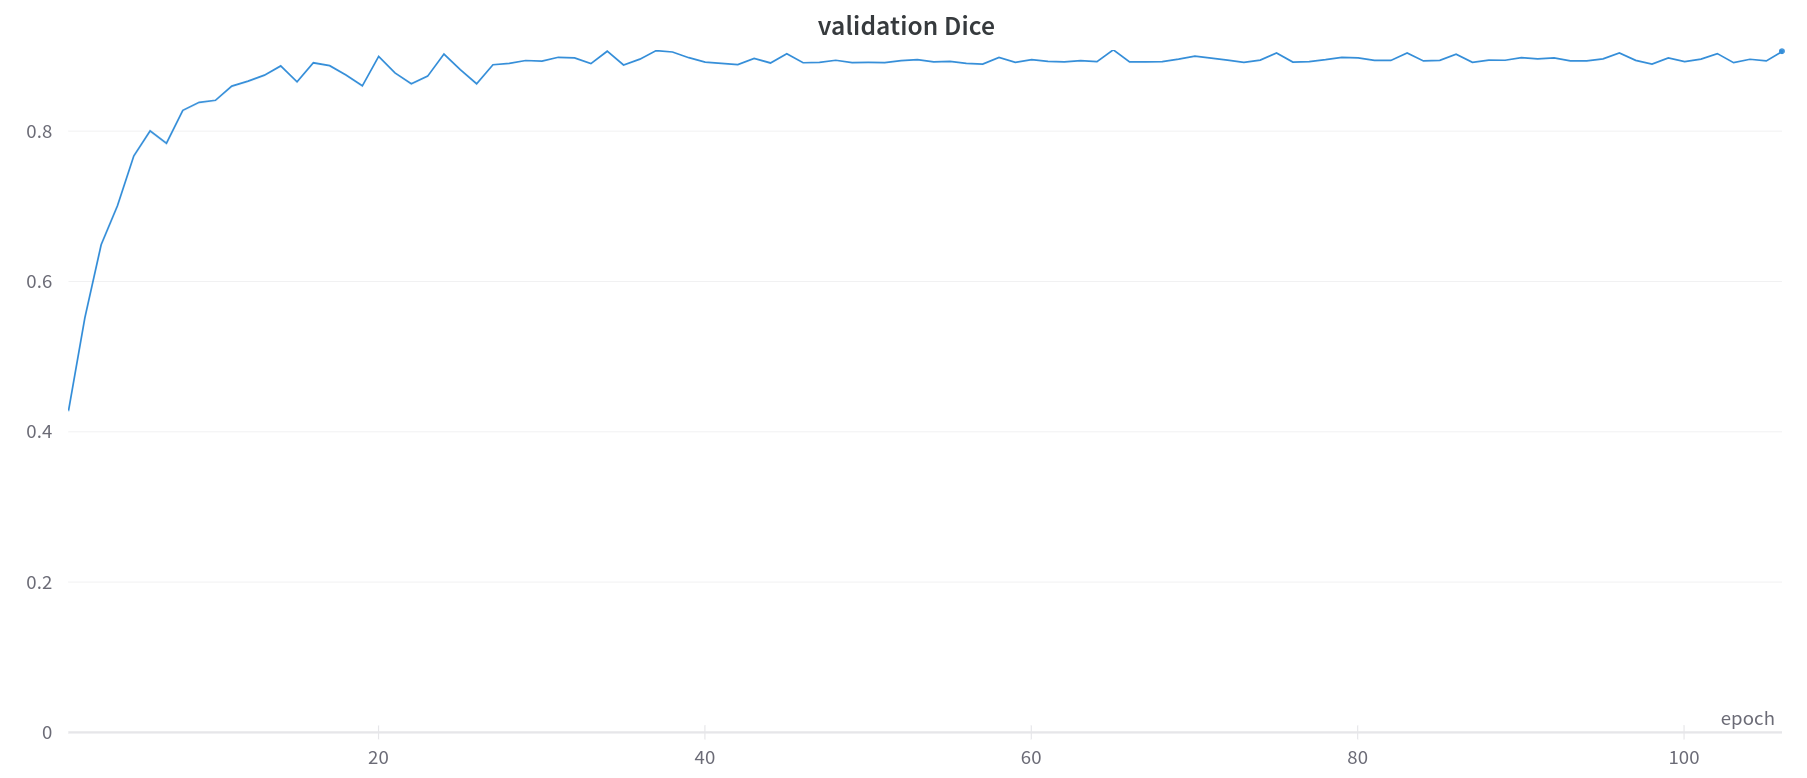
\includegraphics[width=12cm]{images/unet/castros_copy.png}
\caption{Evolution of dice index for hillforts copy paste dataset}
\end{figure}

\begin{figure}[H]
\centering
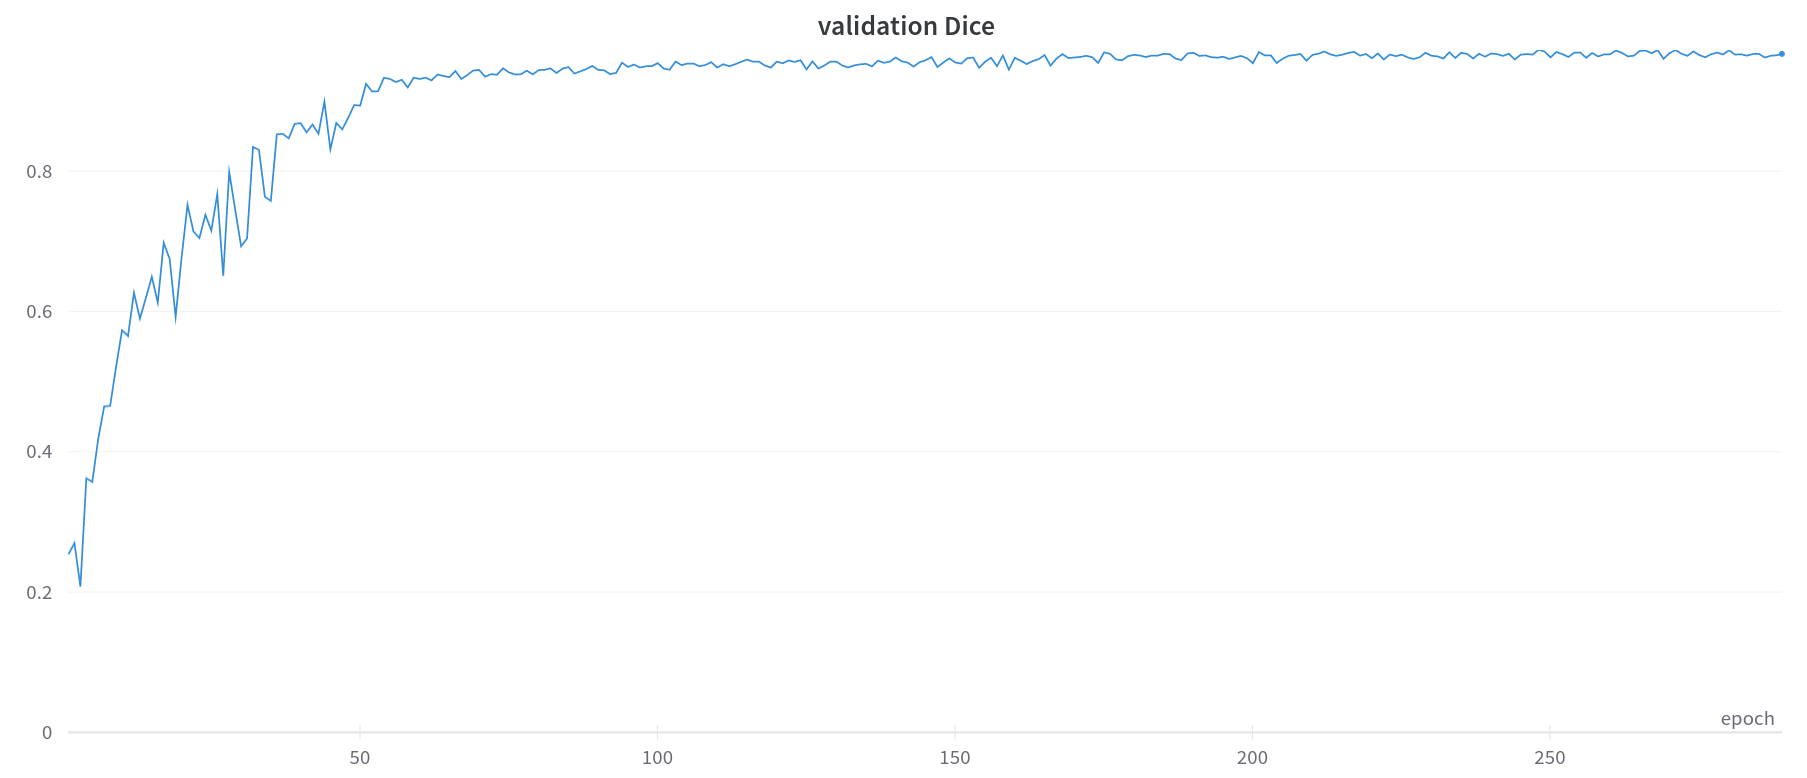
\includegraphics[width=12cm]{images/unet/castros_simple.png}
\caption{Evolution of dice index for hillforts simple dataset}
\end{figure}

As we can see, all training sessions stabilized with a validation dice around 80\%.

One value that was fundamental to the training of the models was the learning rate. The default learning rate was 0.001, but it was verified that with this value the model still hadn't started to converge after almost 50 epochs, even a reduction of the learning rate in 10\% was programmed if there was no improvement after 5 seasons. Several values were tried, finally 1e-7 was chosen.

For unet it was not possible to train with the unaugmented dataset, because most likely the dataset is small, the model had not started to converge after 100 epochs for both the tumuli and the hillforts.


\subsection{Inference}

The same script used in YOLO was employed for inferring the four LRM images. A sliding window of 640x640 pixels was created, with a sliding factor of 50\% for tumuli and 30\% for hillforts. After that, a crop was performed. In cases where the crop contained potential archaeological zones, this was verified using the land occupation map, and the crop was subsequently processed by the model.

The key distinction in the inference process between Yolo and Unet lies in the subsequent step. Unet generates results in a matrix format, where each element corresponds to a pixel in the image and contains the pixel's classification. To obtain segmentation, the OpenCV function findContours was utilized. This function provides the polynomials that enclose the masks. If a polynomial was not located within areas that cannot be archaeological zones (determined using the land use charter), it was saved for further analysis.

Next, the same YOLO inference function was used to eliminate duplicate results from the sliding window. The remaining outcomes were validated using the Local Outlier Factor (LOF) model. Finally, the annotations were saved in CSV files.

The next tables shows the results from inference, also here was used the same script used in YOLO to analyze the results.

\begin{table}[H]
\centering
\begin{tabular}{|c c c|} 
 \hline
  &  Copy Paste & Simple \\ [0.5ex] 
 \hline\hline
 Total & 621 & 1117 \\ 
 Validations & 378 & 808 \\
 True positives & 121 & 177 \\
 False positives & 500 & 940 \\
 False negatives & 155 & 99\\ [1ex] 
 \hline
\end{tabular}
\caption{Results of inference for tumulis(Unet)}
\end{table}

\begin{table}[H]
\centering
\begin{tabular}{|c c c|} 
 \hline
  & Copy Paste & Simple \\ [0.5ex] 
 \hline\hline
 Total & 267 & 2938 \\ 
 Validations & 98 & 1227\\
 True positives & 135 & 108 \\
 False positives & 132 & 2830 \\
 False negatives & 28 & 55\\ [1ex] 
 \hline
\end{tabular}
\caption{Results of inference for hillforts(Unet)}
\end{table}

As in YOLO, the total is the total number of detections of the model, the validations are the total number of validated results of the LOF model, the true positives, false positives and false negatives are relative to the total number of detections and not to the results validated by the LOF.

As can be seen, the results are quite different from YOLO, the first difference is in the number of detections, Unet has detected many fewer archaeological sites than YOLO, but it has left many of the sites already noted undetected.

\begin{figure}[H]
    \centering
    \subfloat{{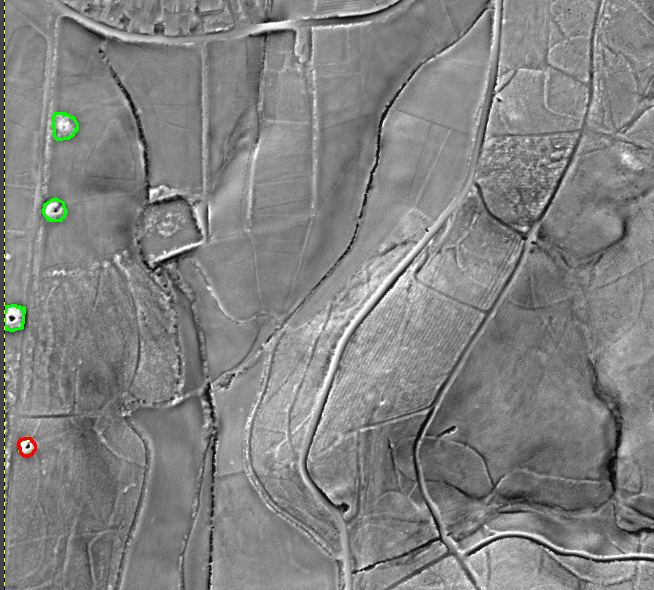
\includegraphics[width=7cm]{images/examples_inference/unet/mamoas/1.png} }}%
    \qquad
    \subfloat{{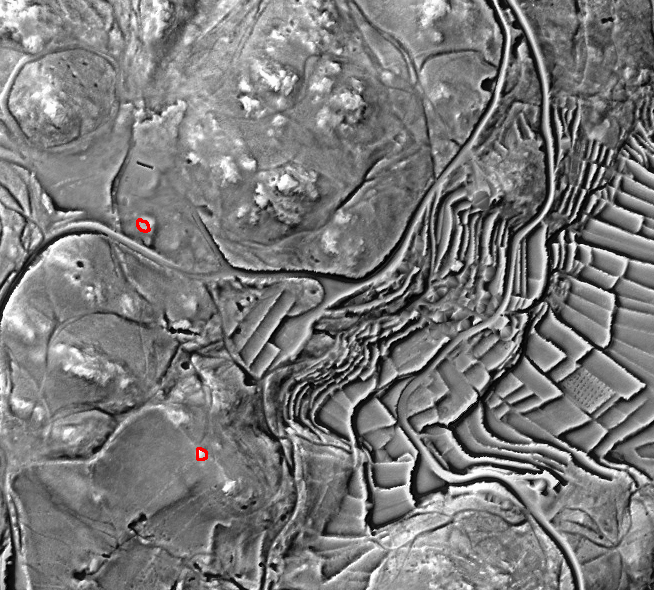
\includegraphics[width=7cm]{images/examples_inference/unet/mamoas/2.png} }}%
    \caption{Examples of inference results from the copy-paste model for tumulis, the green corresponds to a ground truth, while the red corresponds to a detection from Unet.}%
    \label{fig:unet4mamoas}
\end{figure}

In the figures \ref{fig:unet4mamoas} and  \ref{fig:yolo4mamoas} it is possible to see the contrast between false negatives, in Yolo and Unet, while Yolo detected four ground truth tumuli on the left, Unet detected only one.

\begin{figure}[H]
    \centering
    \subfloat{{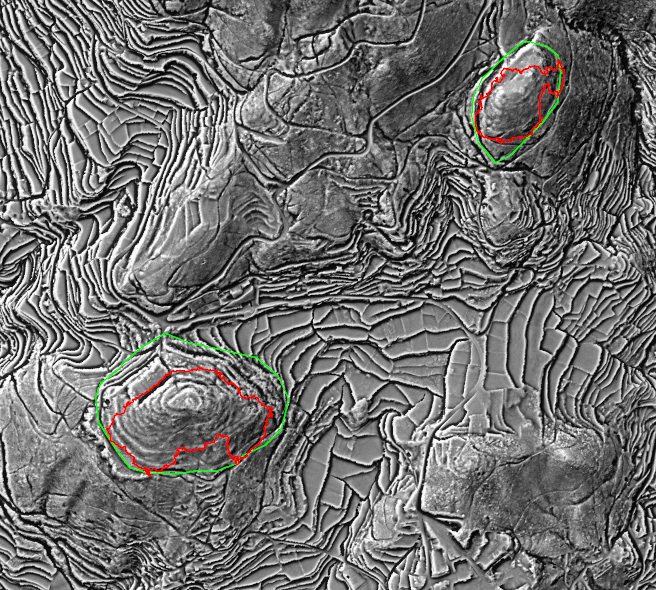
\includegraphics[width=7cm]{images/examples_inference/unet/castros/1.png} }}%
    \qquad
    \subfloat{{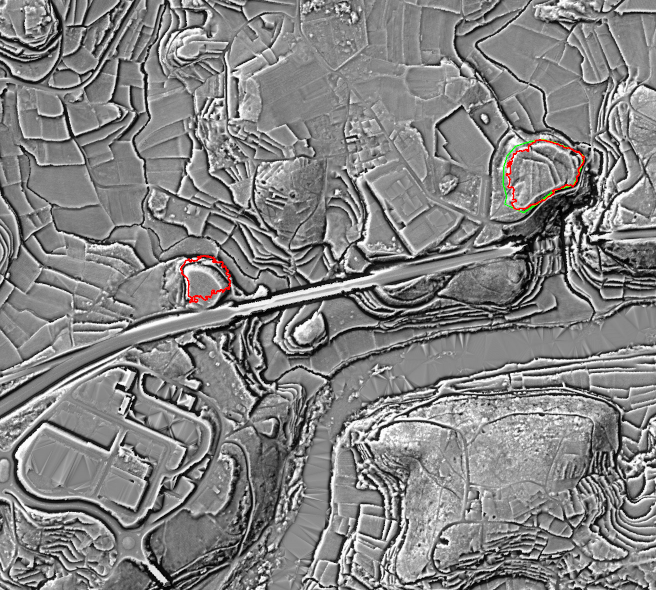
\includegraphics[width=7cm]{images/examples_inference/unet/castros/2.png} }}%
    \caption{Examples of inference results from the copy-paste model for hillforts, the green corresponds to a ground truth, while the red corresponds to a detection from Unet.}%
\end{figure}


\section{Yolov7-seg}
YOLOv7-seg is a modification of YOLOv7, it is an integration of BlendMask with YOLOv7, each bouding box generated by YOLOv7 is then fed into BlendMask neural network in order to generate the segmentation.

\subsection{Model training}

YOLOv7-seg was trained exclusively using the simple dataset. The decision to use this dataset was driven by the superior performance in YOLOv7. Since the primary focus of the project is archaeological site localization rather than segmentation, the results are expected to be quite similar to those of YOLOv7. However, the ability to obtain segmentation could be advantageous for archaeological purposes.


\begin{figure}[H]
    \centering
    \subfloat{{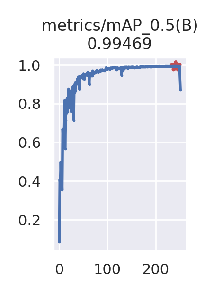
\includegraphics[width=5cm]{images/yoloseg/training/yolosegmamoas.png} }}%
    \qquad
    \subfloat{{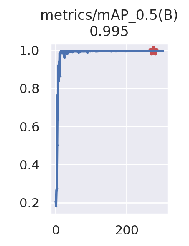
\includegraphics[width=5cm]{images/yoloseg/training/yolosegcastros.png} }}%
    \caption{Results of YOLO-seg for tumulis(left) and hillforts(right)}%
\end{figure}

As can be seen, the training is identical to YOLOv7 training (figure \ref{fig:tumuliyolomaia} and figure \ref{fig:hillyolomaia}), for the same dataset, as expected

\subsection{Inference}
In the inference, a script similar to unet's was used, but instead of the model's result format being in table format, the result comes in polynomial format.

The next table shows the results from the YOLOv7-seg inference.

\begin{table}[H]
\centering
\begin{tabular}{|c c c|} 
 \hline
  &  Tumulis & Hillforts \\ [0.5ex] 
 \hline\hline
 Total & 1410 & 1624 \\ 
 Validations & 1009 & 553 \\
 True positives & 213 & 90 \\
 False positives & 1197 & 1534 \\
 False negatives & 63 & 73\\ [1ex] 
 \hline
\end{tabular}
\caption{Results of inference(YOLO-seg)}
\end{table}

As expected, the results are not much different from YOLOv7.